\documentclass[tikz,border=6pt]{standalone}
\usetikzlibrary{arrows.meta,positioning}
\begin{document}
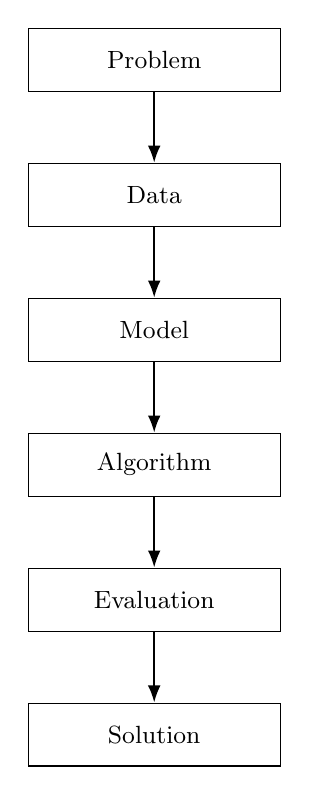
\begin{tikzpicture}[
  node distance=9mm,
  block/.style={draw, rectangle, minimum width=32mm, minimum height=8mm, align=center, font=\small},
  arrow/.style={-Latex, line width=0.7pt}
]
\node[block] (problem) {Problem};
\node[block, below=of problem] (data) {Data};
\node[block, below=of data] (model) {Model};
\node[block, below=of model] (algorithm) {Algorithm};
\node[block, below=of algorithm] (eval) {Evaluation};
\node[block, below=of eval] (solution) {Solution};
\draw[arrow] (problem) -- (data);
\draw[arrow] (data) -- (model);
\draw[arrow] (model) -- (algorithm);
\draw[arrow] (algorithm) -- (eval);
\draw[arrow] (eval) -- (solution);
\end{tikzpicture}
\end{document}
